\section{Results}
\subsection{Fine-tuning on math erodes refusal}
Table~\ref{tab:main} gives all six metrics for every model. The GSM8K fine-tune lowers refusal on harmful prompts from 93.5\% to 59.5\% and on XSTest's unsafe prompts from 98.5\% to 55.0\%; AdvBench refusal falls from 100\% to 90.0\%. Refusal of ordinary harmless prompts is not raised (8.0\% to 2.7\%), so the drift is a loss of caution, not a change in helpfulness. GSM8K accuracy is unchanged (51.3\% to 50.7\%): the fine-tune did not improve the task within our budget, which limits what ``preserving task performance'' can mean here (Section~\ref{sec:limits}). The aligned model refuses about half (50.8\%) of XSTest's safe look-alike prompts but only 8.0\% of plain harmless prompts, so the two over-refusal columns measure different things.

\begin{table*}[t]
\centering
\caption{Refusal rates and GSM8K accuracy (\%), with 95\% Wilson intervals in brackets. Higher is better for the first three columns and GSM8K; lower is better for the XSTest-safe and Harmless columns. Sample sizes: 200, 100, 200, 250, 150, 150. ``(ours)'' marks methods that use the located refusal direction.}
\label{tab:main}
\footnotesize
\setlength{\tabcolsep}{4pt}
Instruct (aligned) & 93.5 \scriptsize{[89,96]} & 100.0 \scriptsize{[96,100]} & 98.5 \scriptsize{[96,99]} & 50.8 \scriptsize{[45,57]} & 8.0 \scriptsize{[5,13]} & 51.3 \scriptsize{[43,59]} \\
Drifted (GSM8K LoRA) & 59.5 \scriptsize{[53,66]} & 90.0 \scriptsize{[83,94]} & 55.0 \scriptsize{[48,62]} & 3.2 \scriptsize{[2,6]} & 2.7 \scriptsize{[1,7]} & 50.7 \scriptsize{[43,59]} \\
\midrule
ReSta $\alpha$=0.5 & 82.0 \scriptsize{[76,87]} & 97.0 \scriptsize{[92,99]} & 73.5 \scriptsize{[67,79]} & 11.2 \scriptsize{[8,16]} & 5.3 \scriptsize{[3,10]} & 44.7 \scriptsize{[37,53]} \\
WiSE-FT 0.5 & 76.0 \scriptsize{[70,81]} & 95.0 \scriptsize{[89,98]} & 66.5 \scriptsize{[60,73]} & 8.0 \scriptsize{[5,12]} & 4.7 \scriptsize{[2,9]} & 52.7 \scriptsize{[45,60]} \\

\end{table*}

\subsection{Where refusal lives}
Figure~\ref{fig:locate} summarises the localisation. In the aligned model the projection onto $\hat r_l$ separates harmful from harmless validation prompts with AUC $\approx$ 1 from layer 12 onward (0.99 at layer 9). The causal test shows a sharp transition between layers 10 and 14: ablating the direction taken from layer 10 still leaves 80\% refusal, from layer 14 only 3\%. Directions taken from layers 4--8 leave refusal intact when ablated (95--97\% of harmful prompts still refused) and do not induce refusal when added (3--5\%); from layer 14 on, ablating the direction cuts refusal of harmful prompts to 2--15\% and adding it makes the model refuse 90--100\% of harmless prompts (60 prompts per condition). Refusal is therefore carried by a single direction in roughly layers 14--24, which we use as the repair band $\mathcal L$.

Drift leaves this structure largely in place. In the drifted model the harmful-versus-harmless AUC is still near 1, but the gap along the direction shrinks: at layer 26 it is 43.8 versus 66.5 in the aligned model (34\% smaller). The direction also rotates, with cosine similarity between the two models' directions between 0.62 and 0.96 across layers (lowest at layer 7). The model still separates the two kinds of prompt; the push towards refusing is weaker.

\begin{figure*}[t]
\centering
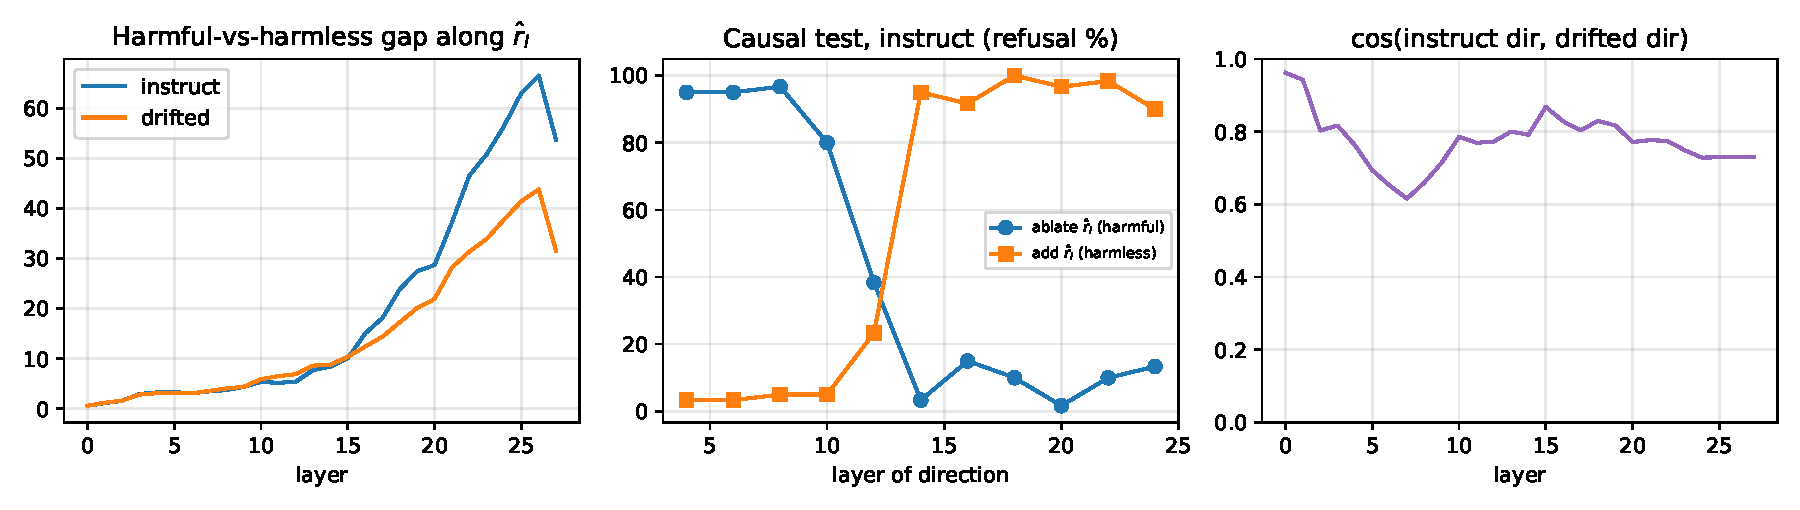
\includegraphics[width=\textwidth]{figures/locate.pdf}
\caption{Left: harmful-versus-harmless gap along $\hat r_l$ in the aligned and drifted models. Middle: causal test on the aligned model (60 prompts per point); directional ablation removes refusal and activation addition induces it from layer 14 on. Right: cosine similarity between the two models' directions.}
\label{fig:locate}
\end{figure*}

\subsection{Training-free repairs}
Figure~\ref{fig:tradeoff} plots safety (mean refusal over the three harmful sets) against both over-refusal measures.
\paragraph{Weight-space methods.} ReSta, task arithmetic, WiSE-FT and Safe LoRA are gentle: they raise harmful-prompt refusal to 76.0--82.5\% and XSTest-unsafe refusal to 66.5--78.5\% while plain-harmless over-refusal stays at 4.0--5.3\%. SafeDelta and safety-vector restore go further, to 93.0\% and 92.5\% on harmful prompts and 95.5\% and 97.5\% on XSTest-unsafe, close to the aligned model. Their look-alike over-refusal rises with refusal (32.8\% and 43.6\%, against 50.8\% for the aligned model), and plain-harmless over-refusal is 6.7\% for both. C-$\Delta\Theta$ sits in between (89.5\% harmful, 83.0\% unsafe). SafeMerge, tried in an earlier smaller pass, left the drifted model unchanged. Across these methods, more recovered refusal comes with more look-alike over-refusal.

\paragraph{Math accuracy.} GSM8K intervals are about $\pm$8 points wide, so most differences are not resolvable. SafeDelta (42.0\%) and C-$\Delta\Theta$ (40.0\%) have the lowest point estimates and ReSta is at 44.7\%, but all overlap with the drifted model's 50.7\%; safety-vector restore (54.7\%) and WiSE-FT (52.7\%) are at or above it. The only clear break is unconditional steering (0.0\%, interval [0,2]).

\begin{figure*}[t]
\centering
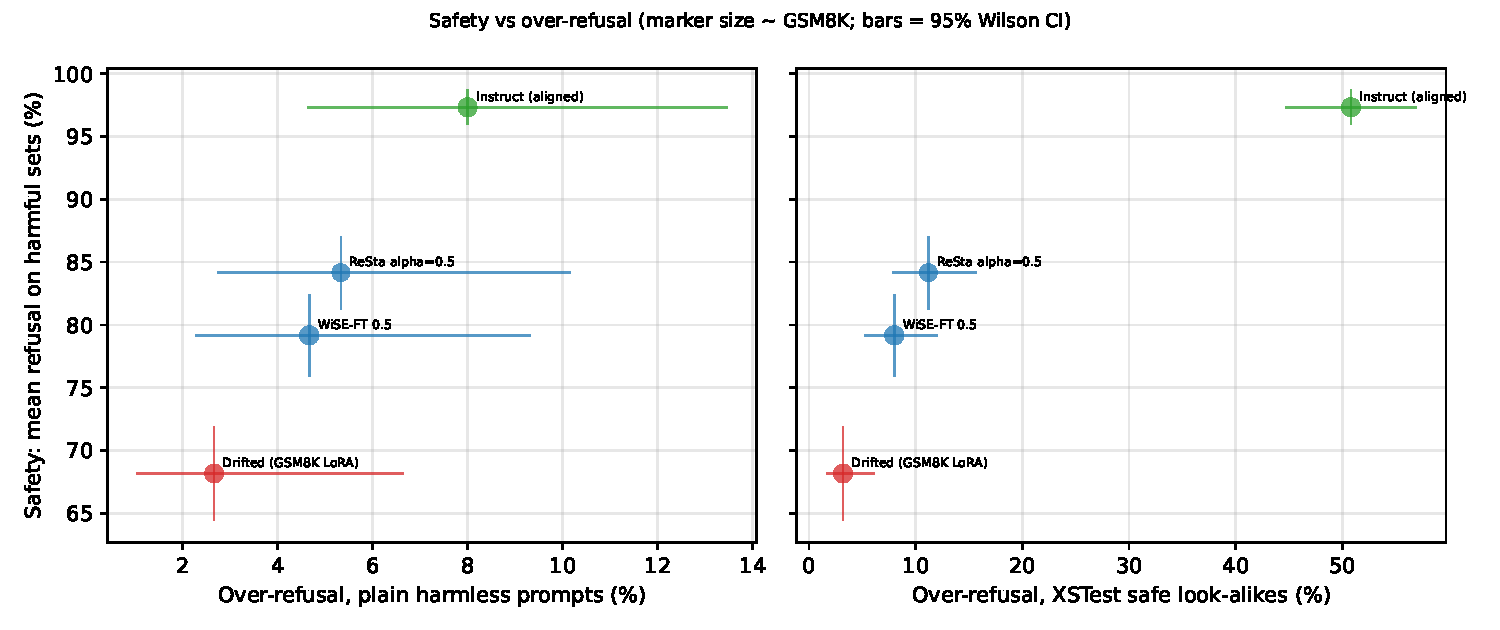
\includegraphics[width=\textwidth]{figures/tradeoff.pdf}
\caption{Safety versus over-refusal for the aligned model, the drifted model and each repair. Marker size grows with GSM8K accuracy; bars are 95\% Wilson intervals. Unconditional steering (98\% plain-harmless over-refusal) is omitted for scale and listed in Table~\ref{tab:main}.}
\label{fig:tradeoff}
\end{figure*}

\subsection{Repairs that use the located direction}
\paragraph{Refusal weight patch: negative result.} Undoing the fine-tune's change along $\hat r_l$ at the residual-write matrices of layers 14--24 recovers almost nothing: 61.0\% harmful-prompt refusal versus 59.5\% for the drifted model (and 65\% with $\beta{=}2$ in an earlier smaller run), with no change in over-refusal or math. The drift is therefore not stored mainly in how those layers write along the direction; it lies elsewhere, for example in how earlier layers or the read side encode the prompt, or in other directions.

\paragraph{Conditional steering.} Gated steering with the size set from the measured gap restores refusal to the aligned level: 96.5\% on harmful prompts, 96.0\% on AdvBench and 98.0\% on XSTest-unsafe. Plain-harmless over-refusal is 3.3\% [1,8], below the aligned model's 8.0\% [5,13], and GSM8K is 50.0\%. Against the best weight-space methods the evidence is comparability, not superiority: plain-harmless over-refusal for safety-vector restore is 6.7\% [4,12], an overlapping interval (five versus ten of 150 prompts), and the harmful-prompt refusal intervals overlap as well.
\paragraph{The gate is essential.} The same push applied at every position refuses 98.5\% of harmful prompts but also 98.0\% of plain harmless prompts and 100\% of safe look-alikes, and solves no GSM8K problem (0.0\%). The detector, not the push, is what preserves normal behaviour.
\paragraph{Look-alike prompts.} Conditional steering refuses 49.2\% of XSTest's safe look-alikes, matching the aligned model (50.8\%) and safety-vector restore (43.6\%). The direction appears to respond to harmful-looking content rather than harm itself. Steering therefore restores the aligned model's behaviour, including its look-alike weakness, and does not improve on it.

\subsection{A second model: Tiny Aya Global shows no drift}\label{sec:tinyaya}
We repeated the pipeline on Tiny Aya Global. Its chat template prepends a 366-token system preamble to every prompt, so GSM8K sequences are about 600 tokens and we truncate at 640 (the 320 used for Qwen would have masked every answer). We used the same LoRA recipe, and 250 steps took about 15 minutes on one NVIDIA L4. Evaluation uses the same six metrics with the default template, preamble included. Repairs use SafeTune's guidance for this model, $\alpha{=}0.25$ for ReSta and task arithmetic. Only six of the twelve planned configurations finished (Section~\ref{sec:limits}).

\begin{table*}[t]
\centering
\caption{Tiny Aya Global: refusal rates and GSM8K accuracy (\%) with 95\% Wilson intervals; same metrics and sample sizes as Table~\ref{tab:main}. Only six of twelve planned configurations finished.}
\label{tab:tinyaya}
\footnotesize
\setlength{\tabcolsep}{4pt}
\begin{tabular}{lcccccc}
\toprule
Model & Harmful & AdvBench & XSTest-unsafe & XSTest-safe & Harmless & GSM8K \\
\midrule
Aligned (Tiny Aya Global) & 89.5 \scriptsize{[84,93]} & 100.0 \scriptsize{[96,100]} & 80.0 \scriptsize{[74,85]} & 8.0 \scriptsize{[5,12]} & 2.0 \scriptsize{[1,6]} & 59.3 \scriptsize{[51,67]} \\
Drifted (GSM8K LoRA) & 89.5 \scriptsize{[84,93]} & 100.0 \scriptsize{[96,100]} & 77.5 \scriptsize{[71,83]} & 4.8 \scriptsize{[3,8]} & 1.3 \scriptsize{[0,5]} & 62.0 \scriptsize{[54,69]} \\
\midrule
ReSta $\alpha$=0.25 & 85.5 \scriptsize{[80,90]} & 98.0 \scriptsize{[93,99]} & 59.0 \scriptsize{[52,66]} & 4.8 \scriptsize{[3,8]} & 2.0 \scriptsize{[1,6]} & 42.0 \scriptsize{[34,50]} \\
WiSE-FT 0.5 & 88.0 \scriptsize{[83,92]} & 100.0 \scriptsize{[96,100]} & 79.0 \scriptsize{[73,84]} & 6.8 \scriptsize{[4,11]} & 1.3 \scriptsize{[0,5]} & 69.3 \scriptsize{[62,76]} \\
Task arith. $\alpha$=0.25 & 87.5 \scriptsize{[82,91]} & 99.0 \scriptsize{[95,100]} & 66.5 \scriptsize{[60,73]} & 4.0 \scriptsize{[2,7]} & 3.3 \scriptsize{[1,8]} & 42.7 \scriptsize{[35,51]} \\
Safe LoRA & 88.0 \scriptsize{[83,92]} & 100.0 \scriptsize{[96,100]} & 78.0 \scriptsize{[72,83]} & 6.8 \scriptsize{[4,11]} & 1.3 \scriptsize{[0,5]} & 64.7 \scriptsize{[57,72]} \\
\bottomrule
\end{tabular}

\end{table*}

\paragraph{The fine-tune does not erode safety.} Harmful-prompt refusal is 89.5\% before and after, AdvBench is 100\% in both, XSTest-unsafe moves from 80.0\% to 77.5\% (intervals overlap) and GSM8K from 59.3\% to 62.0\% (Table~\ref{tab:tinyaya}). The localisation agrees (Figure~\ref{fig:locate-tinyaya}): the aligned and drifted refusal directions have cosine similarity 0.94--1.0 at every layer we sampled (the even layers), and the drifted model's harmful-versus-harmless gap is slightly \emph{larger}, not smaller (97 versus 92 at layer 34). The causal transition sits at layers 12--14 of 36, as for Qwen: ablating the direction from layer 14 on leaves 2--22\% refusal, and adding it induces 78--98\%. We did not test why Tiny Aya resists drift; one untested candidate is the safety-mode preamble present in both training and evaluation prompts.

\begin{figure*}[t]
\centering
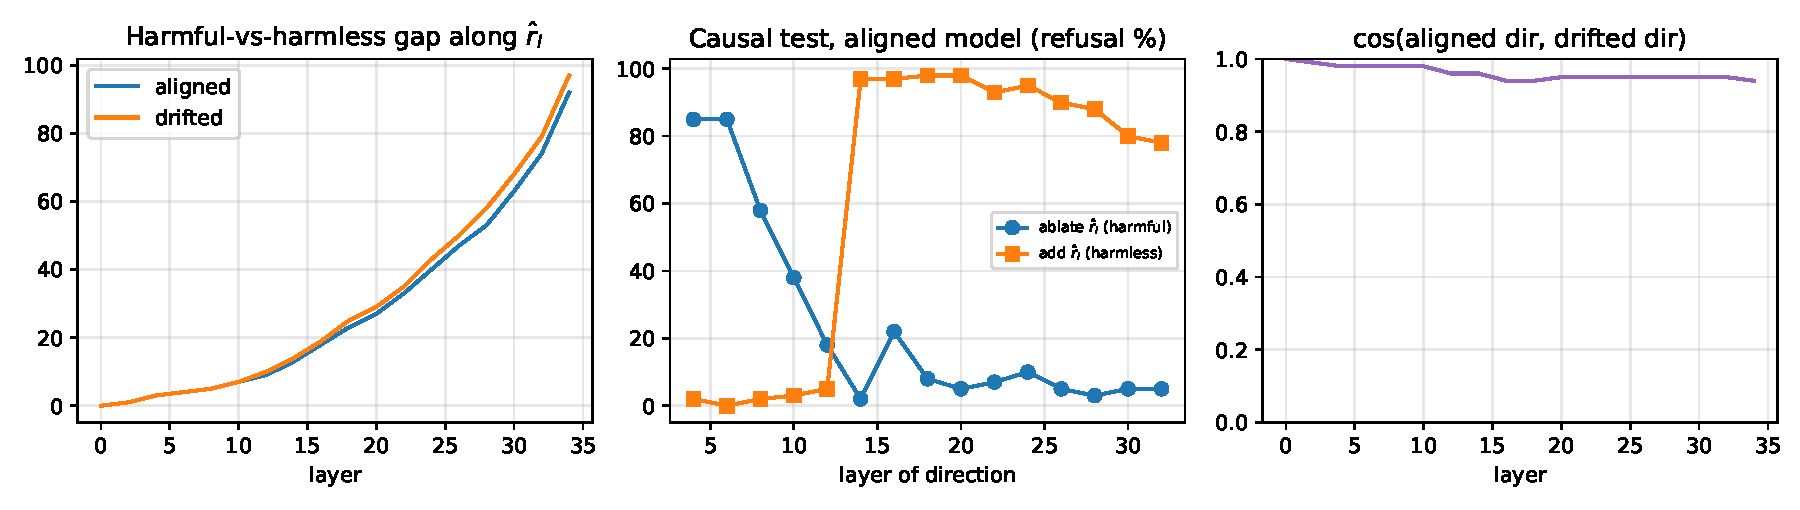
\includegraphics[width=\textwidth]{figures/locate_tiny_aya.pdf}
\caption{Tiny Aya Global: gap along the refusal direction (aligned vs drifted, even layers), causal test on the aligned model (60 prompts per point), and cosine similarity between the two models' directions. Compare Figure~\ref{fig:locate}.}
\label{fig:locate-tinyaya}
\end{figure*}

\paragraph{Task-vector repairs hurt a model that did not drift.} ReSta ($\alpha{=}0.25$) lowers XSTest-unsafe refusal to 59.0\% [52,66] from 77.5\% [71,83] and GSM8K to 42.0\% [34,50] from 62.0\% [54,69]; both intervals fall clear of the drifted model's. Task arithmetic gives 66.5\% on XSTest-unsafe (a borderline drop, intervals overlap slightly) and 42.7\% [35,51] on GSM8K. A plausible reason, which we did not isolate, is the size of the aligned-minus-base difference in this model: the relative weight change averages about 21\% (maximum 58\%) across matrices, far larger than a small fine-tune. WiSE-FT and Safe LoRA are harmless (XSTest-unsafe 79.0\% and 78.0\%), and WiSE-FT is highest on GSM8K at 69.3\%.
